% Este archivo es parte de la memoria del proyecto fin de carrera
% de Manuel López Urbina. Protegida bajo la licencia GFDL.
% Para más información, la licencia completa viene incluida en el
% fichero fdl-1.3.tex

% Copyright (C) 2017 Manuel López Urbina

\newpage

\begin{appendix}
\backmatter

\chapter{Anexos}
\label{appendix:anexos}


Anexos con las instrucciones para la instalación de todos los componentes software empleados en el desarrollo del proyecto.\\

\section{Instalación de Node.js}


Instalación de los prerrequisitos:\\

\begin{lstlisting}[language=bash]
sudo apt-get install python-software-properties python g++ make
\end{lstlisting}


Si está utilizando Ubuntu 16.04, necesitará hacer los siguiente:\\

\begin{lstlisting}[language=bash]
sudo apt-get install software-properties-common
\end{lstlisting}


Añadimos el repositorio:\\

\begin{lstlisting}[language=bash]
sudo add-apt-repository ppa:chris-lea/node.js
\end{lstlisting}

Actualizamos la lista de paquetes:\\

\begin{lstlisting}[language=bash]
sudo apt-get update
\end{lstlisting}

Instalación de  Node.js:\\

\begin{lstlisting}[language=bash]
sudo apt-get install nodejs
\end{lstlisting}




\section{Instalación Sails.js}

Esta guía proporciona las pautas necesarias para la configuración de un entorno de trabajo para el desarrollo de aplicaciones Sails. Esta guía no cubre la instalación de en un entorno de producción.\\

\subsection{Prerrequisitos}

Partiendo de que se encuentra Node.js correctamente instalado en una máquina con Ubuntu 16.04.2 LTS. Ubuntu es una plataforma muy popular y utilizada en el desarrollo de Sails.js, al igual que otros sistemas operativos basados en Unix, como Mac OS X. La instalación es relativamente fácil y existe multitud de información gracias a su amplia comunidad de desarrolladores.\\

\begin{itemize}

\item{Una máquina con Ubuntu 16.04.2 LTS }
\item{Node js instalado.}


\end{itemize}

\subsection{Instalación}

A continuación detallaremos los pasos para la instalación de Sails. Lo primero que haremos es instalar Sails haciendo uso de npm, el gestor de paquetes que viene con el propio Node. Para ello, lo que vamos a hacer es ir directamente a la terminal y e introducir lo siguiente:\\

\begin{lstlisting}[language=bash]
sudo npm install sails -g
\end{lstlisting}

La opción -g, qe significa global, lo que hace es instalar Sails a nivel global, la cual nos permitirá acceder a las funcionalidades de Sails que emplearemos para la creación de nuestros proyectos.\\

Es posible que necesite permisos de administrador para instalar Sails a nivel global.\\

Para comprobar que la instalación se realizó correctamente, crearemos un proyecto inicial y levantaremos el servidor. Para ello introducimos en la terminal:\\

\begin{lstlisting}[language=bash]
sails new my_first_app
\end{lstlisting}

Cambiamos de directorio (cd) al nuevo directorio creado, en el cual nos aseguraremos de que Sails está correctamente instalado. Para ello arrancaremos el servidor y comprobaremos en nuestro navegador en localhost 1337 (localhost: 1337) que Sails está funcionando correctamente.\\


\begin{lstlisting}[language=bash]
cd my_fisrt_app
sails lift
\end{lstlisting}


Tras introducir en nuestro navegador \emph{localhost: 1337} debemos obtener el siguiente resultado:


\begin{figure}[H]
  \begin{center}
    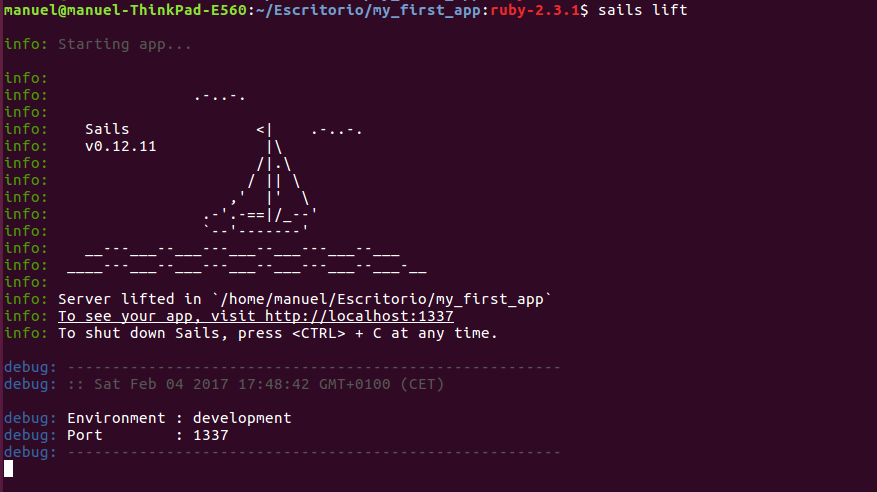
\includegraphics[scale=0.3]{imagenes/running_sails.png}
  \end{center}
  \label{fig:logo}
 \caption{Iniciando Sails.}
\end{figure}


Y en nuestro navegador:\\

\begin{figure}[H]
  \begin{center}
    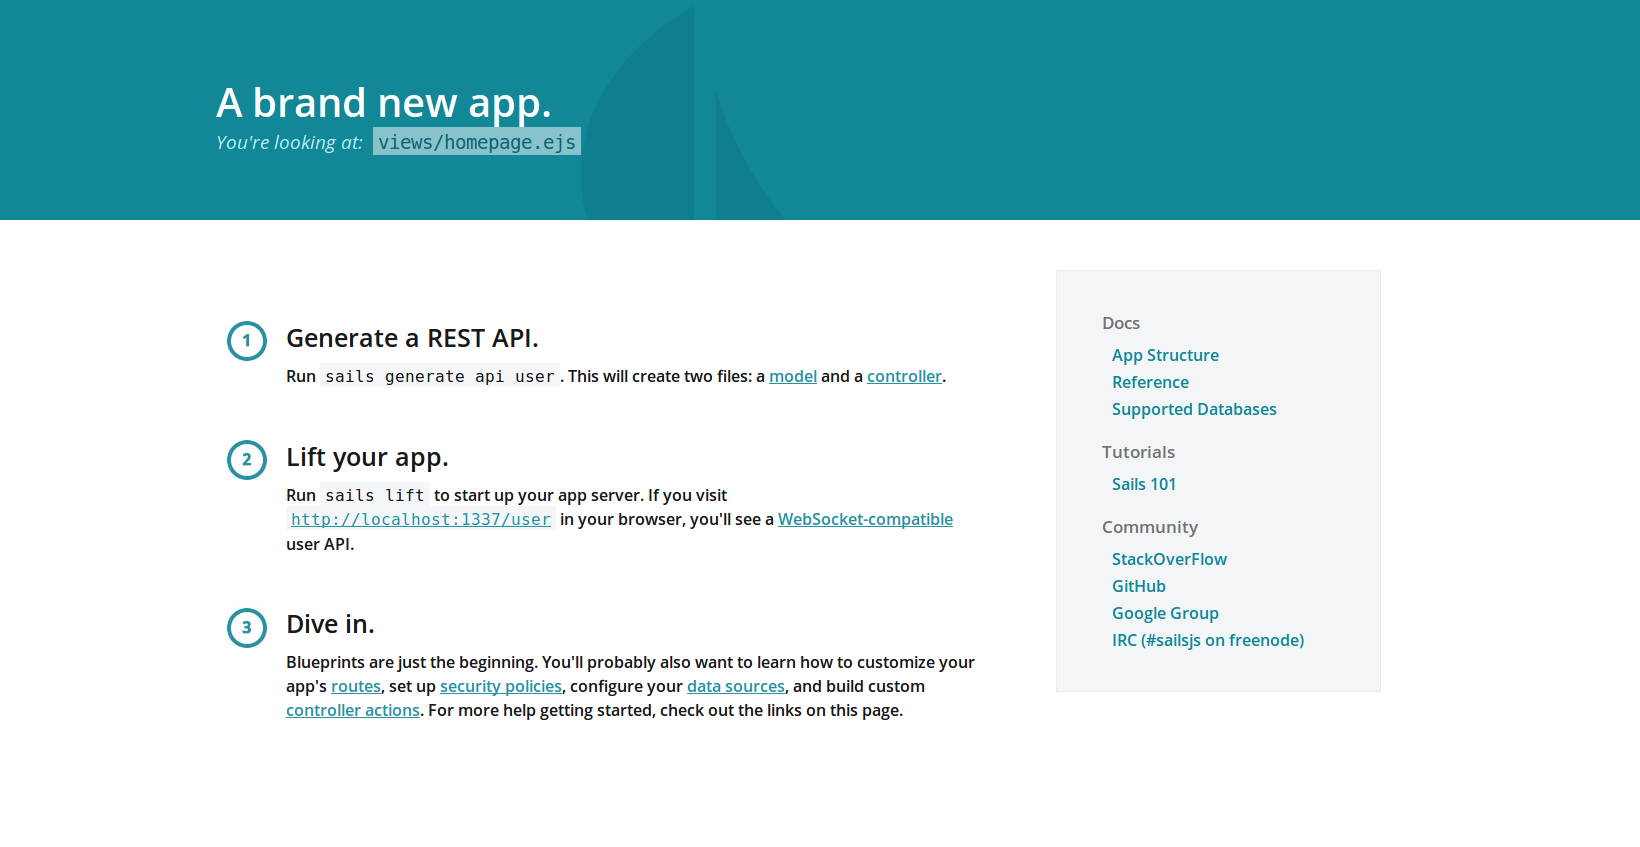
\includegraphics[scale=0.3]{imagenes/browser_sails.png}
  \end{center}
  \label{fig:logo}
 \caption{Sails en funcionamiento \protect\footnotemark.}
\end{figure}



\section{Instalación de MongoDB}

MongoDB es una base de datos libre y de código abierto NoSQL utilizada comúnmente en aplicaciones web modernas. Esta guía le ayudará a configurar MongoDB en su máquina para un entorno de aplicación de producción.\\

\subsection{Prerrequisitos}

Para seguir esta guía es necesario:
\begin{itemize}

\item{Una máquina con Ubuntu 14.04.}
\item{Un usuario con permisos de administrador (no root).}
\end{itemize}

\subsection{Instalación}


Para la instalación de MongoDB se puede optar con la versión disponible en los repositorios de paquetes de Ubuntu a pesar de que no sea la última versión disponible. Los repositorios propios de MongoDB proporcionan
la versión más actualizada siendo la forma recomendada de instalación. Para la instalación desde repositorios externos, Ubuntu garantiza la autenticidad de los paquetes de software al verificar que están firmados
con las claves GPG, por lo que primero tenemos que importar la clave para el repositorio oficial de MongoDB.\\

Para ello, debemos ejecutar:\\

\begin{lstlisting}[language=bash]
sudo apt-key adv --keyserver hkp://keyserver.ubuntu.com:80 --recv 7F0CEB10
\end{lstlisting}


Después de importar con éxito la clave, obtendremos el siguiente:\\

\begin{lstlisting}[language=bash]
Gpg: Número total procesado: 1
Gpg: importado: 1 (RSA: 1)
\end{lstlisting}

A continuación, tenemos que actualizar los detalles del repositorio de MongoDB para que APT sepa de dónde descargar los paquetes.\\

Introduzca el siguiente comando para crear un archivo de lista para MongoDB.\\

\begin{lstlisting}[language=bash]
echo "deb http://repo.mongodb.org/apt/ubuntu "\$(lsb_release -sc)"/mongodb-org/3.0 multiverse" | sudo tee /etc/apt/sources.list.d/mongodb-org-3.0.list
\end{lstlisting}

Después de agregar los detalles del repositorio, necesitamos actualizar la lista de paquetes.\\

\begin{lstlisting}[language=bash]
sudo apt-get update
\end{lstlisting}


Ahora podemos instalar el propio paquete MongoDB.\\

\begin{lstlisting}[language=bash]
sudo apt-get install -y mongodb-org
\end{lstlisting}

Este comando instalará varios paquetes que contengan la última versión estable de MongoDB junto con útiles herramientas de administración para el servidor MongoDB.\\

Después de la instalación del paquete, MongoDB se iniciará automáticamente. Puede comprobarlo ejecutando el siguiente comando.\\

\begin{lstlisting}[language=bash]
service mongodb status
\end{lstlisting}

Si MongoDB se está ejecutando, se mostrará una salida como la siguiente (con un ID de proceso diferente).\\

\begin{lstlisting}[language=bash]
 mongodb.service - An object/document-oriented database
   Loaded: loaded (/lib/systemd/system/mongodb.service; enabled; vendor preset: enabled)
   Active: active (running) since sáb 2017-02-04 13:07:01 CET; 11h ago
     Docs: man:mongod(1)
 Main PID: 807 (mongod)
    Tasks: 10
   Memory: 84.8M
      CPU: 4min 7.494s
   CGroup: /system.slice/mongodb.service
            - 807 /usr/bin/mongod --config /etc/mongodb.conf
\end{lstlisting}

También es posible detener, iniciar y reiniciar MongoDB utilizando los siguientes comandos:\\

\begin{lstlisting}[language=bash]
service mongodb stop
service mongodb start
\end{lstlisting}


\section{Instalación del control de versiones Git}

Para seguir esta guía es necesario disponer de una máquina con Ubuntu 14.04.\\

La forma más sencilla de tener Git instalado y configurado para su utilización es mediante el uso de los repositorios predeterminados de Ubuntu. 
Este es el método más rápido, pero, por contra puede ser que la versión disponible no sea la más reciente. 
Si necesita la última versión, deberá seguir los pasos para compilar Git desde el origen.\\

Si no necesitamos disponer de la última versión podemos instalarlo desde el repositorio de Ubuntu. Para ello introducimos los siguientes comandos en una terminal:\\

\begin{lstlisting}[language=bash]
sudo apt-get update
sudo apt-get install git
\end{lstlisting}

Esto descargará e instalará Git en el sistema. A continuación se describe los pasos para su configuración.

\subsection{Configuración}

Una vez que disponemos de Git instalado, necesitamos realizar una serie de pasos para añadir nuestros datos de acceso de nuestro repositorio.\\

La forma más sencilla de hacerlo es a través del comando \emph{git config} proporcionando nuestro nombre y dirección de correo electrónico. Esto es debido a que Git incorpora esta información en cada commit
que hacemos. Por ejemplo, si nuestro nombre es \emph{RobotUI} y nuestro email \emph{email@robotui.com}, los comandos de configuración serían los siguientes:\\

\begin{lstlisting}[language=bash]
 git config --global user.name "RobotUI"
 git config --global user.email "email@robotui.com"
\end{lstlisting}

Finalmente podemos comprobar todos los valores de configuración establecidos escribiendo:\\

\begin{lstlisting}[language=bash]
git config --list
\end{lstlisting}

Existen muchas más opciones configurables pero estos son los dos esenciales necesarios.\\

\section{Despliegue de una aplicación Sails}

Para el despliegue de la aplicación se a empleado una serie de herramientas y procedimientos que se encuentran recogidos en el recurso bibliográfico \cite{book:Deploying}, una referencia de gran 
utilidad para la puesta en producción de aquellas aplicaciones desarrolladas en cualquier framework Node.js. Caso del presente proyecto.\\

A continuación se describe una guía elemental, la cual ha sido seguida para la puesta en producción de RobotUI y que ha sido elaborada a partir de la citada referencia.\\

Primeramente, debemos definir el entorno de producción para nuestra aplicación Sails. Para ello editamos el fichero \emph{/config/env/production.js} introduciendo los siguientes datos:\\

\begin{itemize}
 \item Nombre de nuestra conexión de la base de datos la cual hemos definido en nuestro archivo \emph{config/connections.js}
 \item Dirección IP de nuestro servidor.
 \item Puerto por el que queremos correr nuestra aplicación.
\end{itemize}
  
Un ejemplo de configuración es el siguiente:

\begin{lstlisting}[language=JavaScript]
/**
 * Production environment settings
 *
 * This file can include shared settings for a production environment,
 * such as API keys or remote database passwords.  If you're using
 * a version control solution for your Sails app, this file will
 * be committed to your repository unless you add it to your .gitignore
 * file.  If your repository will be publicly viewable, don't add
 * any private information to this file!
 *
 */

module.exports = {

  /********************************************************************
   * Set the default database connection for models in the production *
   * environment (see config/connections.js and config/models.js )    *
   ********************************************************************/

  models: {
    connection: 'MongodbServer'
  },

  /********************************************************************
   * Set the port in the production environment to 80                 *
   ********************************************************************/

  port: 1337,

  /********************************************************************
   * Set the log level in production environment to "silent"          *
   ********************************************************************/

  log: {
    level: "silent"
  }

  proxyHost: '46.101.102.33',
  proxyPort: 1337

};
\end{lstlisting}

En el servidor de producción se ha utilizado Nginx \footnote{Nginx es un servidor web/proxy inverso ligero de alto rendimiento y un proxy para protocolos de correo electrónico (IMAP/POP3)} 
con la siguiente configuración:\\

\begin{lstlisting}[language=bash]

server {
  listen        80;
  server_name   46.101.102.33;


   listen 443 ssl;

   ssl_certificate /etc/nginx/ssl/nginx.crt;
   ssl_certificate_key /etc/nginx/ssl/nginx.key;

   location / {
        proxy_pass         http://46.101.102.33:1337/;

	proxy_http_version 1.1;
	proxy_set_header Upgrade $http_upgrade;
	proxy_set_header Connection "upgrade";
	proxy_set_header Host $host;

    }

}

\end{lstlisting}

Para arrancar la aplicación, se ha hecho uso del gestor de procesos Pm2, se introduce la siguiente orden: \\

\begin{lstlisting}[language=bash]
  sudo pm2 start app.js -x -- --prod
\end{lstlisting}


Para monitorizar la aplicación, Pm2 incorpora una herramienta de gestión de procesos. Para visualizarlo introducimos en una terminal:\\

\begin{lstlisting}[language=bash]
  sudo pm2 monit
\end{lstlisting}


Obteniendo un resultado similar al siguiente:

\begin{figure}[H]
  \begin{center}
    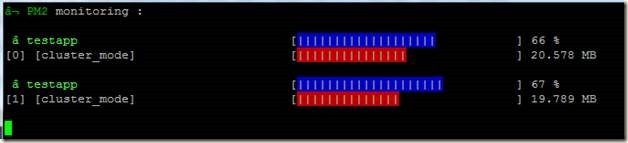
\includegraphics[scale=0.8]{imagenes/pm2-monit.jpg}\\
    \caption{Utilización del gestor de procesos Pm2 en el entorno de producción.}
  \end{center}
\end{figure}



\end{appendix}





